\chapter{Reconstructor}
\label{sec:reconst} 

The reconstructor associates all available target reports to unique targets, each identifed by a \textbf{U}nique \textbf{T}arget \textbf{N}umber (\textbf{UTN}). For each of the targets, reference trajectories ("optimal" position estimates akin to system track updates) are calculated and written to the database. \\

Reference trajectories are calculated based on available sensors and System Trackers, as selected by the user. \\

2 different reconstructors exist, but the advanced reference trajection calculation feature (Probabilistic + IMM Reconstructor) is only available under a commercial professional license. In the free license, a basic reconstructor (Scoring + UMKalman) is available. Please refer to \nameref{sec:ui_configure_licenses} for licensing information. \\

\begin{itemize}  
   \item Basic: Scoring + UMKalman
   \begin{itemize}  
   \item Included in free version
   \item Association based on secondary attributes and simple, configurable distance scoring
   \item Position estimation using Linear Uniform Motion Kalman filter
   \end{itemize}  
   \item Advanced: Probabilistic + IMM
   \begin{itemize}  
   \item Requires commercial professional license
   \item Association based on secondary attributes and self-adaptive probabilistic thresholds
   \item Uses Radar bias estimation \& correction, ADS-B geometric altitude for slant range correction, accuracy re-estimation and scaling, ADS-B verification, ...
   \item Position estimation using Interacting Multiple Models (IMM) filter, with a Rauch-Tung-Striebel (RTS) smoother
   \end{itemize}
\end{itemize}  

For optimal performance, the processing of the target reports and reconstruction is time-sliced. In (commonly) 15 minute intervals, all target reports are loaded, associated to UTNs, references are calculated and written to the database, after which the next time-slice is loaded. \\

In the 'Probabilistic + IMM' reconstructor, each data slice is processed multiple times, to re-estimate correctable bias' as well as to rescale target report accuracies. \\

\subfile{reconstructor_config}

\section{Workflow}
For each processed slice, the following general steps are performed:

\begin{itemize}
\item Load all target reports for the current time-slice
\item Remove all target reports / calculated information for the previous time-slice
\item Load all target reports, per data source
\item Associate target reports to UTNs
   \begin{itemize}  
   \item If possible, associate by matching reliable secondary attribute
    \begin{itemize}  
    \item Mode S Address, Mode S Identification, Reliable Track Number
    \end{itemize}
   \item Otherwise, associate by matching Mode A/C and position
   \item Otherwise, associate by position only
   \end{itemize}
\item Self-associate new targets (find matching UTNs created by the same target)
\item Retry-Associate target reports
\item Compute references
\item Calculate statistics based on references
\item Write references \& associations
\end{itemize}
\ \\

There are several algorithmic features of interest, which are described in the following chapters, but deeper discussion is outside the scope of this document.

\subsection{Associate Target Reports to Targets}

The following steps are performed for each target report:
\begin{itemize}
\item Check if association can be made using lookup lists of targets based on
\begin{itemize}
\item Mode S address
\item Mode S identification
\begin{itemize}
\item Ignoring "00000000", "????????", "        " values
\end{itemize}
\item CAT062/Reference Trajectory Track number (data source + line specific)
\end{itemize}
\item Otherwise, associate by matching Mode A/C and position
\item Otherwise, associate by position only
\item If a matching target is found, the best match is used for association
\item If no matching target is found
\begin{itemize}
\item If the target report has Mode S address/identification or a reliable Track Number, a new target is created
\item Otherwise no association is made (stored for later retry-association)
\end{itemize}
\ \\

In case of a match, this match is verified. A match based on the Track Number can e.g. be revoked if the time difference to the last target update is larger than the 'Maximum Track Time Difference' parameter, 
or if the distance threshold is larger than the 'Track Number Disassoc. Distance Factor' parameter, assuming the 'Do Track Number Disassoc. Using Distance' parameter is set. \\

If still valid, the target report is associated to the specific UTN, which in turn updates the respective lookup lists.

\subsubsection{Position Matching}

For considering a position match, a position score is calculated for each target report, to all possible targets. In the case of 'Scoring + UMKalman', the distance offsets (target report to interpolated target position at time of target report) are compared to the 'Maximum Acceptable Offset', and only associated to the best match if within such a distance.

\subsubsection{New Target Creation}

When creating a new target using a target report, the secondary attributes are stored in the lookup lists of targets.

\subsection{Self-associate New Targets}

For all newly created targets, other possibly matching targets are checked if a computed match score would allow merging a target pair. 
This enables merging of created targets even if single target reports (e.g. during the somewhat unstable beginning of tracking) did not allow for it.

\begin{itemize}
\item Associate new per-source targets to existing targets based on
\begin{itemize}
\item Minimum time overlap: 'Minimum Time Overlap Probability' parameter
\item Mode A code(s) similarity
\item Mode C code(s) similarity: 'Maximum Altitude Difference' parameter
\item Position similarity
\begin{itemize}
\item Count number of updates being in different distances: \#Erroneous, \#Dubious, \#Acceptable
\item Minimum number of updates checked: 'Minimum Updates' parameter
\item Associate if probabilities of erroneous and dubious updates are not too high
\end{itemize}
\end{itemize}
\end{itemize}
\ \\

\subsection{Target Type}

A target type is defined based the following information (if available):

\begin{itemize}
\item ADS-B emitter category (ECAT)
\item Vehicle Mode S address list
\item Defined FFTs
\item Reported Altitudes
\end{itemize}

\ \\

It encompasses a type (e.g. aircraft type, vehicle, FFT, ...), and adds information about an average target size, expected movement dynamics and ground only flag - all of which are used during reconstruction. \\

The following target types exist:

\begin{itemize}
\item Unknown: No information
\item By ECAT
\begin{itemize}
\item LightAircraft
\item SmallAircraft
\item MediumAircraft
\item HighVortexLargeAircraft
\item HeavyAircraft
\item HighSpeedManoeuvrable
\item Rotocraft
\item OtherAirborne (Gliders, UAVs, ultralights, lighter-than-air, etc. )
\item Vehicle
\item Obstacle
\end{itemize}
\item Other aircraft, not from ECAT but from Mode C
\begin{itemize}
\item AnyAircraft
\end{itemize}
\item By defined FFTs
\begin{itemize}
\item FFT
\end{itemize}
\end{itemize}

\subsection{Discussion}

The user should be aware that, while this association feature is quite capable, it is still somewhat limited. 
It strongly depends on the correctness of Mode S addresses/identification, as well as the Tracker information (track number, secondary information and position information). 
If this information is erroneous, the created association will be sub-optimal or plainly wrong. \\

Also, when associating non-Mode S target reports a trade-off has to be made for the 'Maximum Acceptable Distance' parameter, 
especially if the target reports are primary-only. The parameter should be set within the limits of Reference/Tracker error plus maximum sensor error (which can still include radar bias'), and the used target separation minima. 
This is of course not well-suited for strongly varied sensors accuracies and separations (e.g. when mixing ground and air surveillance data). \\

\section{Probabilistic + IMM Features}

Without going into detail, in this section a short overview is given over the capabilities of the advanced reconstructor. The main improvements are:

\begin{itemize}
\item Rescaling accuracies
\begin{itemize}
\item Assess / verify accuracy of tracked data sources
\item Assess / verify accuracy of ADS-B position quality indicators, per transponders
\item Estimate radar plot position accuracy
\item Using parameters based models as well as 2D accuracy maps
\end{itemize}
\item Correct Radar bias': Estimate and correct azimuth bias, range bias \& gain
\item Use ADS-B geometric altitude for slant-range correction
\begin{itemize}
\item Method based on published paper: \href{https://doi.org/10.3390/engproc2022028008}{'Usage of Geometric Altitude for Radar Plot Position Improvements' by H. Puhr, MDPI 2022}
\item Use geometric altitudes of ADS-B data for improved slant-range correction (instead of using barometric altitudes)
\end{itemize}
\item Do position outlier checks: Associate outlier positions, but do not use them for reference computation
\begin{itemize}
\item Based on estimated target position estimate accuracy and (re-scaled) target report accuracy
\end{itemize}
\item Use Risky ADS-B: (disabled by default) Estimate ADS-B accuracy of transponders without usable position quality indicators
\begin{itemize}
\item Only usable if 'Rescaling Accuracies' is enabled
\end{itemize}
\item Generally: Do not use static position thresholds, but probabilistic ones
\begin{itemize}
\item Mahalanobis distances based on accuracy estimates
\end{itemize}
\item System Tracker Spline interpolation: Generate 1-second updates to compensate for high-update-rate data sources
\item Advanced reconstruction algorithms for reference reconstruction
\begin{itemize}
\item \textbf{I}nteracting \textbf{M}ultiple \textbf{M}odels (IMM) filter
\item \textbf{R}auch-\textbf{T}ung-\textbf{S}triebel (RTS) smoother
\end{itemize}
\end{itemize}


Resampling of system tracks is enabled in order to obtain similar sample rates for tracker and high-update rate (e.g. ADS-B) data, which reduces a sensor-specific bias of the Kalman filter. 
Cubic B-splines are used to interpolate the tracker target reports in a relaxed way. In case a spline segment deviates too strongly from its interval, a linear interpolation is used instead. \\

\subsection{Radar Plot Position Improvements}

Using the features mentioned above, the 'Correct Radar Bias' and the 'Use ADS-B geometric altitude for slant-range correction' features can for example result in the following real-life position improvements: 
median org (original) error vs. median cor (corrected) error in [meters], for 10 different Radars:

\begin{lstlisting}
Rad1 estimateXYStdDev: median error
	 org avg 70.29 mad 34.20
	 cor avg 65.18 mad 32.13 cnt 6476
Rad2 estimateXYStdDev: median error
	 org avg 59.40 mad 31.81
	 cor avg 48.79 mad 29.69 cnt 22571
Rad3 estimateXYStdDev: median error
	 org avg 136.98 mad 57.03
	 cor avg 65.69 mad 34.90 cnt 25725
Rad4 estimateXYStdDev: median error
	 org avg 73.16 mad 33.48
	 cor avg 62.76 mad 34.57 cnt 26050
Rad5 estimateXYStdDev: median error
	 org avg 102.84 mad 54.71
	 cor avg 95.01 mad 61.07 cnt 27595
Rad6 estimateXYStdDev: median error
	 org avg 65.04 mad 34.69
	 cor avg 63.29 mad 38.70 cnt 30520
Rad7 estimateXYStdDev: median error
	 org avg 120.52 mad 57.49
	 cor avg 60.03 mad 33.67 cnt 34208
Rad8 estimateXYStdDev: median error
	 org avg 132.39 mad 88.92
	 cor avg 123.45 mad 79.81 cnt 33445
Rad9 estimateXYStdDev: median error
	 org avg 114.86 mad 56.14
	 cor avg 75.72 mad 46.94 cnt 35744
Rad10 estimateXYStdDev: median error
	 org avg 71.64 mad 32.46
	 cor avg 47.39 mad 24.76 cnt 39444
\end{lstlisting}

\subsection{Rescaling Accuracies}

Depending on the data source type (ADS-B, MLAT, Radar,Tracker) different accuracy scaling methods are used. The goal is to estimate the optimal target report accuracy, to in turn achieve the optimal reconstruction accuracy. 
Commonly, 2D accuracy maps of varying resolution are used. If per-target-report accuracy is given, scaling factors are used to factor out over/underestimation of the target report accuracy by the data source.

\begin{itemize}
\item For Radars: Use average accuracy 2D map, model average accuracy by regression line as fallback
\item For MLAT/Trackers: Use average accuracy 2D map, estimate scaling factors to rescale the given target report accuracy
\item For ADS-B: Model per-quality-indicator-value accuracies for each transponder, estimate scaling factors to rescale the given target report accuracy
\end{itemize}
\ \\

\subsubsection{2D Map Examples}

A common Radar accuracy map can look as follows, with this particular Radar showing a distinct accuracy decrease in a certain azimuth angle:
\begin{figure}[H]
    \hspace*{-2.5cm}
    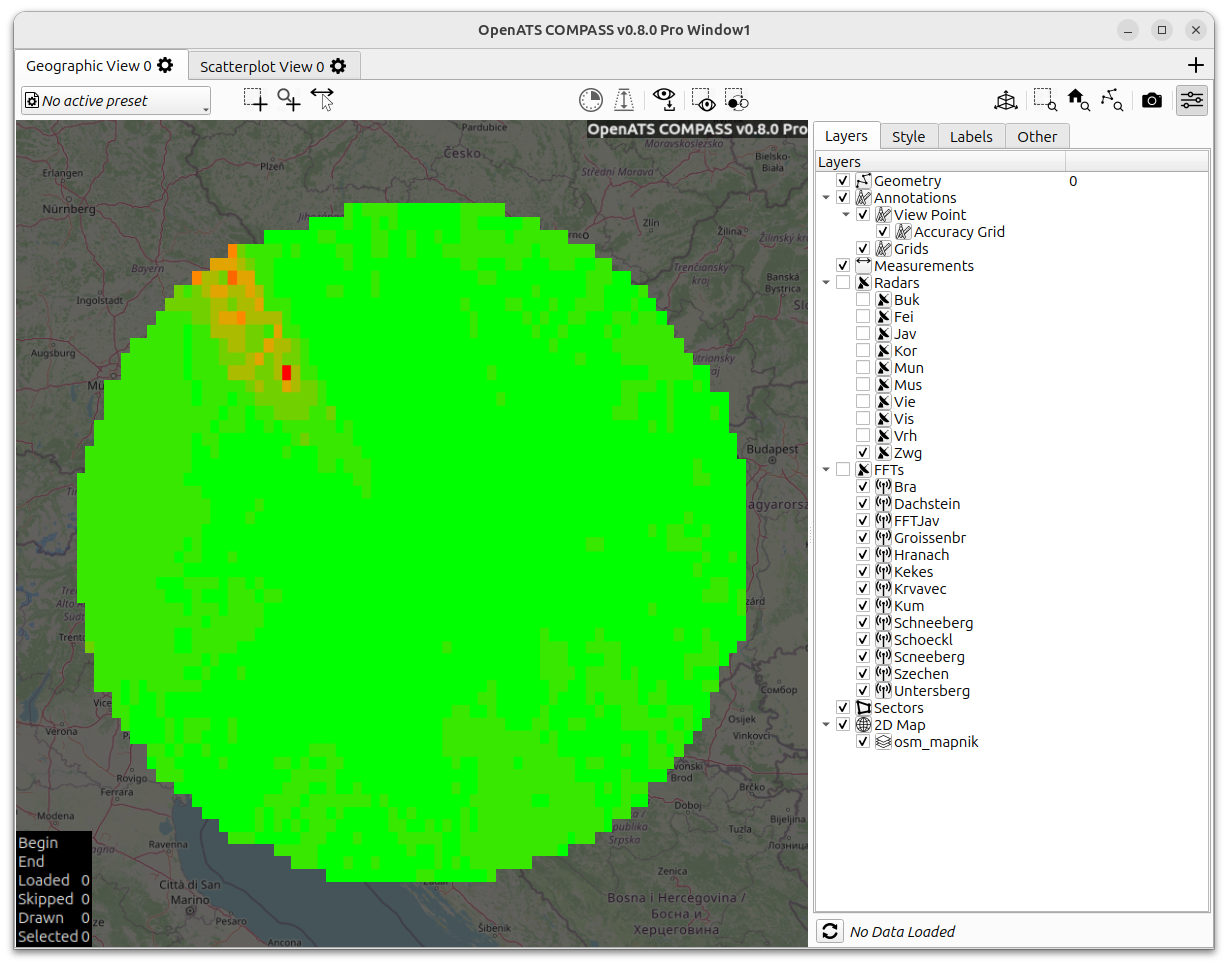
\includegraphics[width=19cm]{figures/radar_acc.png}
  \caption{Radar Accuracy: 0.3m (green) - 2768m (red)} 
\end{figure} 

A common Tracked data source accuracy \textbf{scale factor} map can look as follows, 
with this source showing a distinct accuracy over-estimation (tracking accuracy vs. measured against reconstructed accuracy) in the southern region:
\begin{figure}[H]
    \hspace*{-2.5cm}
    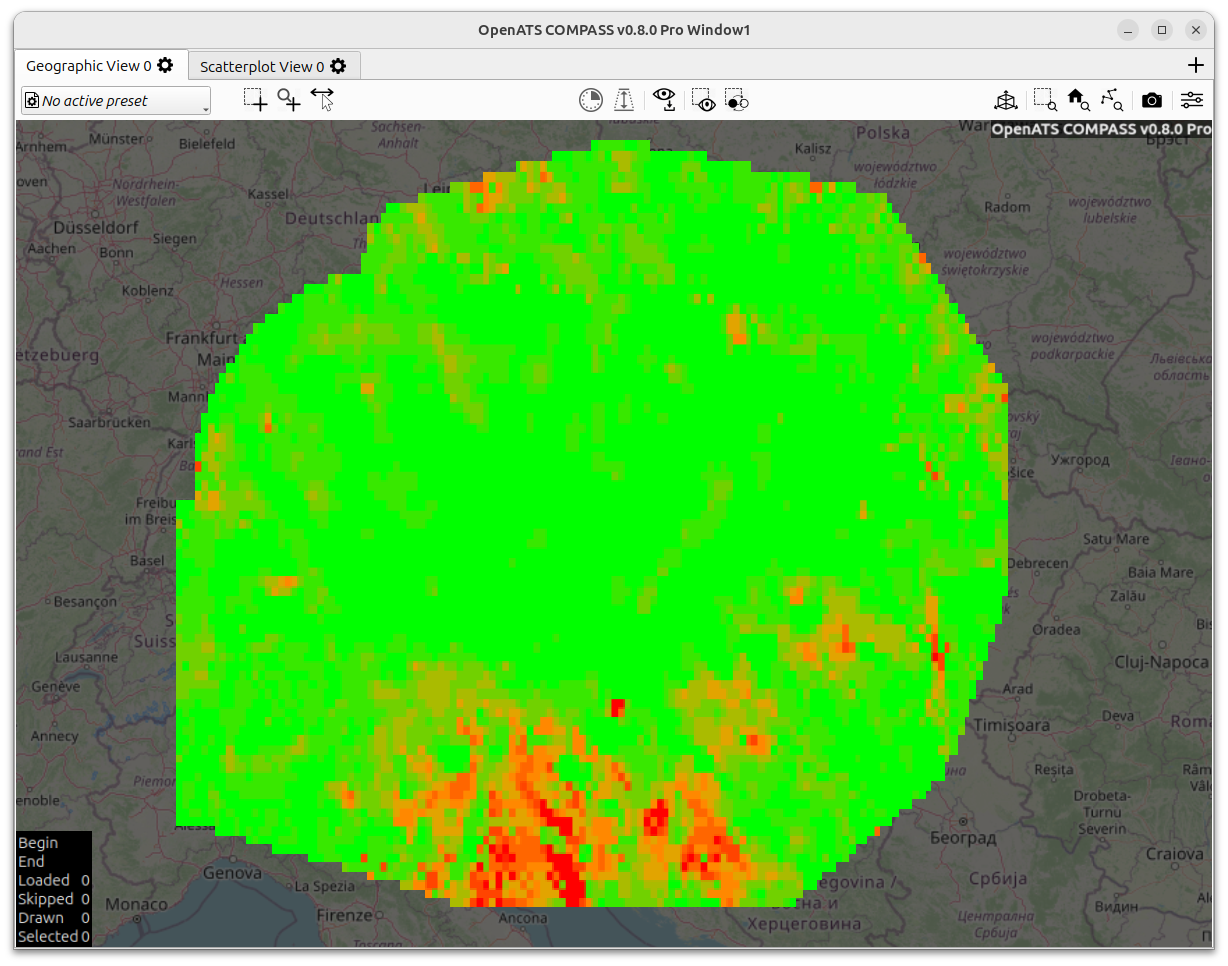
\includegraphics[width=19cm]{figures/tracked_scaling.png}
  \caption{Tracked Source Accuracy Scaling: 0.5 [1] (green) - 5 [1] (red)}
\end{figure} 

The (rescaled) average Tracked data source accuracy map can look as follows, 
showing a nice common accuracy region, with slightly increased errors in some regions (most probably airports) and in the outer limits.
\begin{figure}[H]
    \hspace*{-2.5cm}
    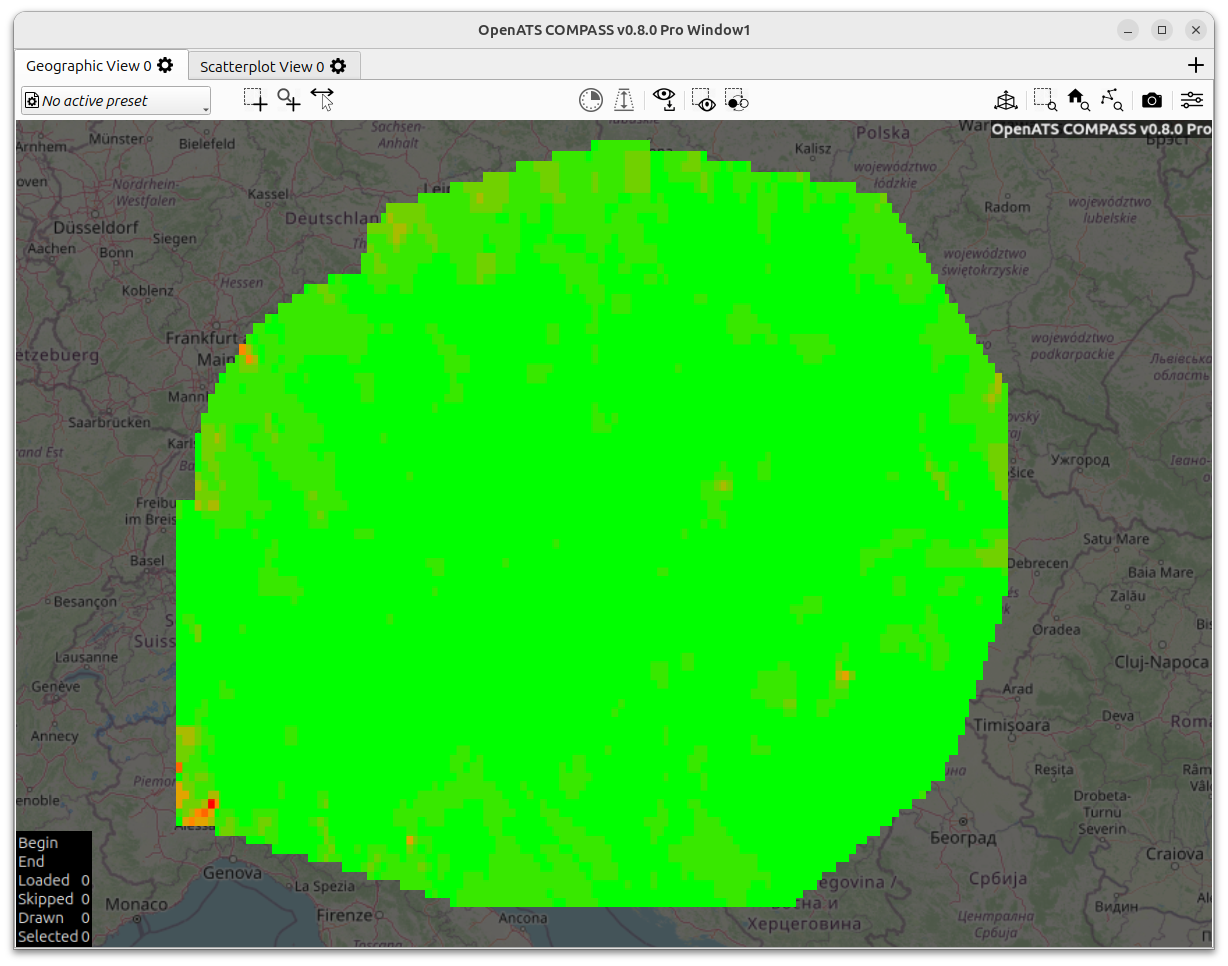
\includegraphics[width=19cm]{figures/tracked_avgerr.png}
  \caption{Tracked Source Average Error Scaling: 1 [m] (green) - 878 [m] (red)}
\end{figure} 

\subsection{Target Example}

\begin{figure}[H]
    \hspace*{-2.5cm}
    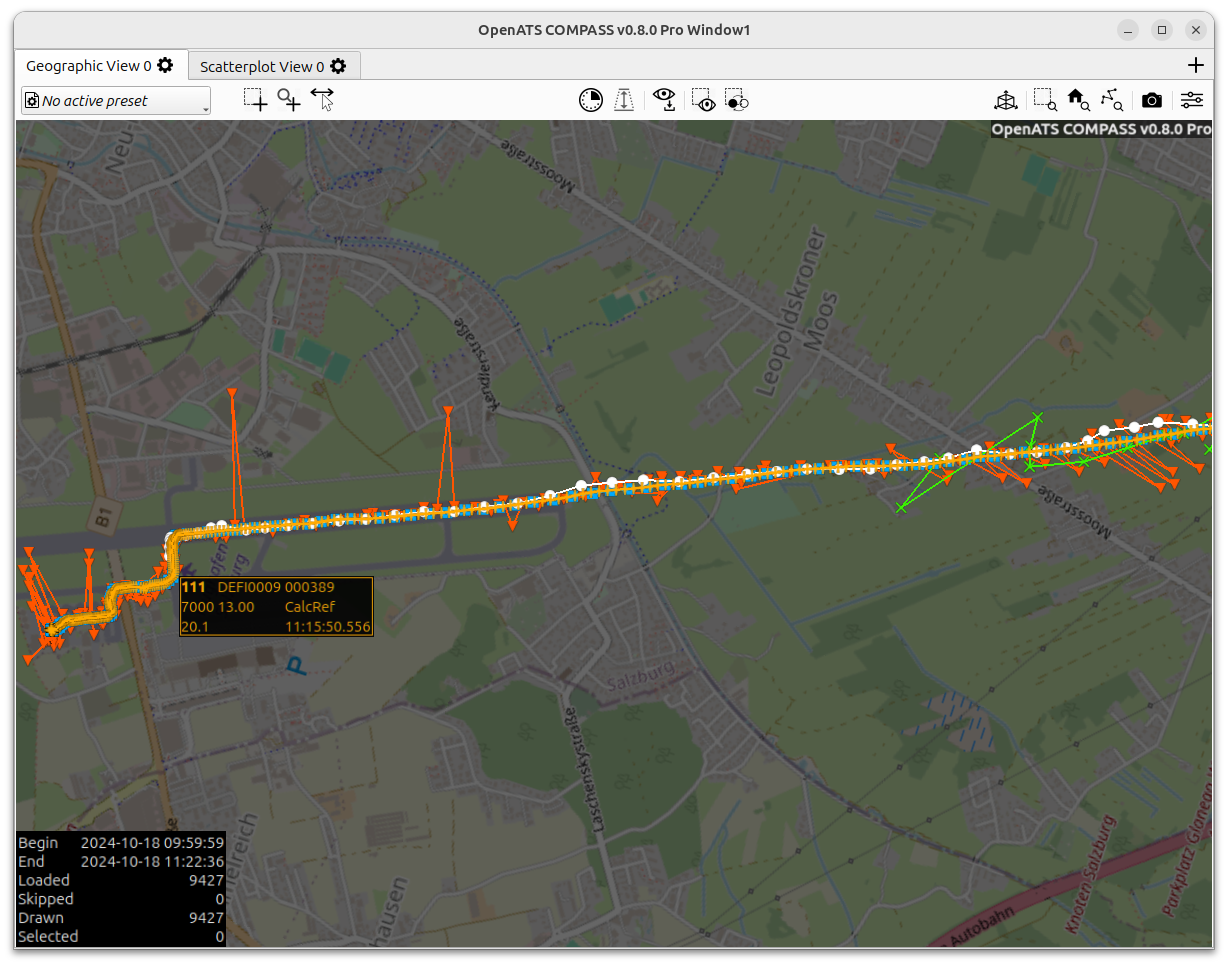
\includegraphics[width=19cm]{figures/target_ex1.png}
  \caption{Reconstructed Target Example}
\end{figure} 

\section{Running}

To run the task, click the 'Run' button. When the task is started, the following progress dialog is shown to the user.

\begin{figure}[H]
    \center
      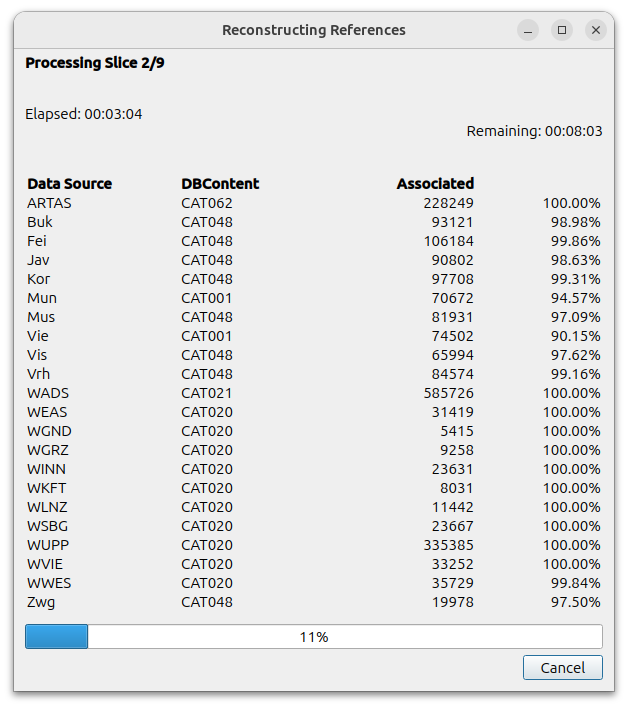
\includegraphics[width=12cm]{figures/process_in_progress.png}
    \caption{Reconstructing References Task - In Progress}
\end{figure}

The processing can be cancelled using the 'Cancel' button, which might take a few seconds. \\

After all data slices are processed and the calculated references associations are saved, the task is done.

\begin{figure}[H]
    \center
      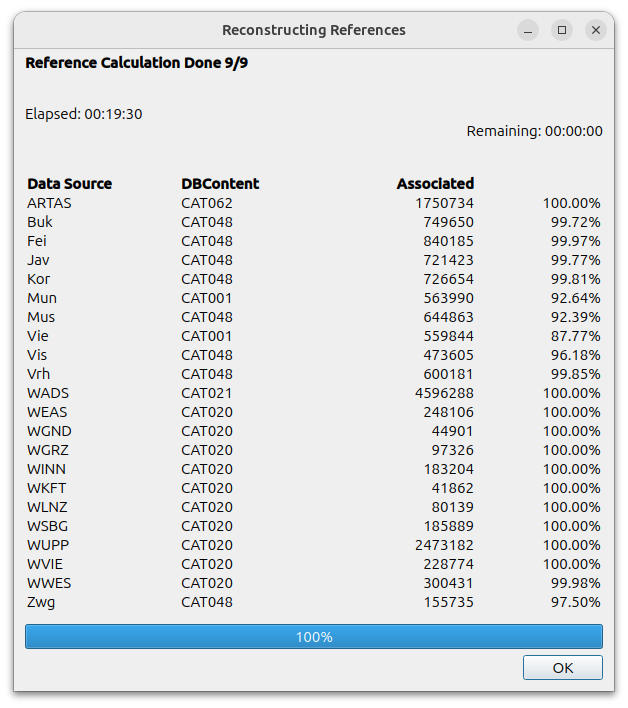
\includegraphics[width=12cm]{figures/process_done.png}
    \caption{Reconstructing References Task - Done}
\end{figure}

After a successful reconstruction, all created unique targets are listed in the main window's 'Targets' tab.

\begin{figure}[H]
    \hspace*{-2.5cm}
    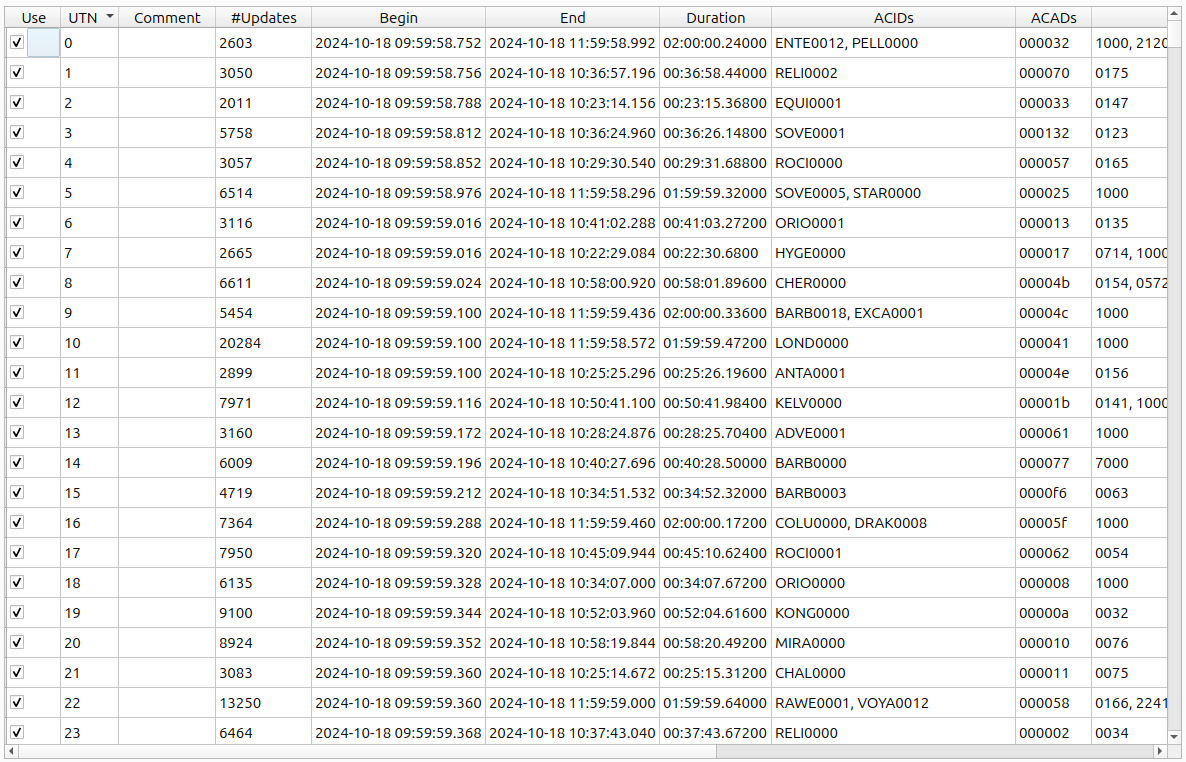
\includegraphics[width=19cm]{figures/created_targets.png}
    \caption{Reconstructing References Task - Created Targets}
\end{figure}
